As análises apresentadas nessa seção resume os resultados dos testes exemplares na extensão feita no Bench4Q, os resultados aqui mostrados são proporcionados como exemplos de aplicação da metodologia, eles não devem ser interpretados como definitivos e avaliações de desempenho. Dessa forma, para uma melhor abordagem dos exemplos apresentados, os exemplo divide-se em 3 partes:
\begin{itemize}
	\item Configuração da carga no Bench4Q
	\item Configuração para modular a carga
	\item Carga gerada
\end{itemize}

\begin{figure}[!htb]
	\begin{subfigure}{\linewidth}
		\centering
		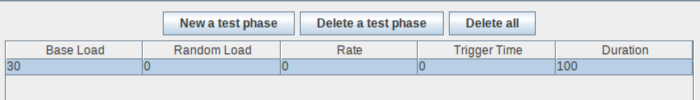
\includegraphics[scale=0.7]{condiguracao-carga-bench4q1.png}
		\caption{Configuração da carga no Bench4Q, para um degrau positivo}
		\label{fig:condiguracao-carga-bench4q1}
	\end{subfigure}\\
	\begin{subfigure}{\linewidth}
		\centering
		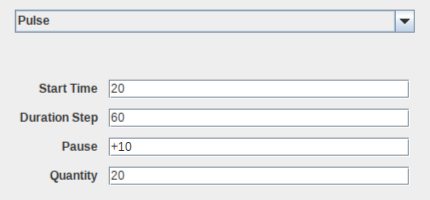
\includegraphics[scale=0.7]{condiguracao-carga-modulada1.png}
		\caption{Configuração para modular a carga como um degrau positivo}
		\label{fig:condiguracao-carga-modulada1}
	\end{subfigure}\\[1ex]
	\begin{subfigure}{\linewidth}
		\centering
		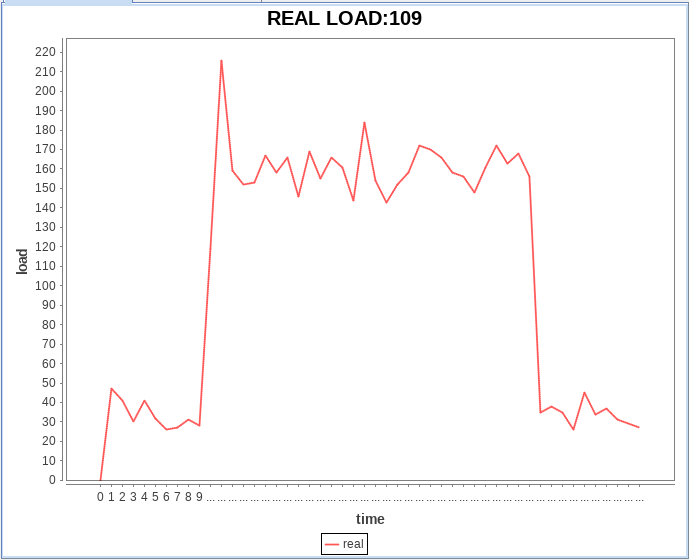
\includegraphics[scale=0.6]{grafico-carga-modulada1.png}
		\caption{Carga gerada com base nas configuração}
		\label{fig:grafico-carga-modulada1}
	\end{subfigure}
	\caption{Carga gerada com base na configuração: Degrau Positivo}
	\label{fig:carga-modulada1}
	\fautor
\end{figure}

A figura \ref{fig:carga-modulada1} apresenta a primeira exemplificação gerada com o Bench4Q já com a extensão desenvolvida neste trabalho, na figura \ref{fig:condiguracao-carga-bench4q1} demonstra os parâmetros de configuração utilizados para gerar a carga, dois são os principiais, \textit{Base Load} e \textit{Duration}, o primeiro define a quantidade e EBs envolvidos nos experimento, neste caso 30 EBs, já o segundo define o tempo de duração do experimento em segundos, neste caso 100 segundos. Na figura \ref{fig:condiguracao-carga-modulada1} são apresentados os parâmetros para modular a carga \textit{Start Time} de valor 20, refere-se ao tempo de esperara para o inicio do restante da carga se mostrar presente e ativa na modulação, assim decorrido 20 segundos os 20, dos 30 EBs, definido pelo \textit{Quantity} iniciam a gerar carga para o sistema, essa carga se manterá ativa durante 60 segundos conforme fixado no parâmetro \textit{Duration Step}, neste exemplo o parâmetro \textit{Pause} não apresentar influencia devido ao seu valor 0.
O resultado pode ser apreciado pela figura \ref{fig:grafico-carga-modulada1}, este gráfico é nativo do próprio Bench4Q, que demonstra o comportamento da carga no decorrer do tempo. Apesar da estocasticidade a carga se modulou conforme programada, essa estocasticidade é característica do Bench4Q, afim de manter um comportamento mais realístico com os de clientes acessando uma estocasticidade \textit{E-commerce}.

\begin{figure}[!htb]
	\begin{subfigure}{\linewidth}
		\centering
		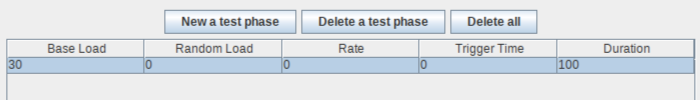
\includegraphics[scale=0.7]{condiguracao-carga-bench4q2.png}
		\caption{Configuração da carga no Bench4Q, para um degrau negativo}
		\label{fig:condiguracao-carga-bench4q2}
	\end{subfigure}\\
	\begin{subfigure}{\linewidth}
		\centering
		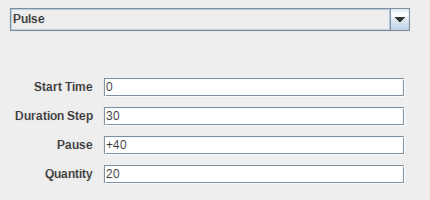
\includegraphics[scale=0.7]{condiguracao-carga-modulada2.png}
		\caption{Configuração para modular a carga como um degrau negativo}
		\label{fig:condiguracao-carga-modulada2}
	\end{subfigure}\\[1ex]
	\begin{subfigure}{\linewidth}
		\centering
		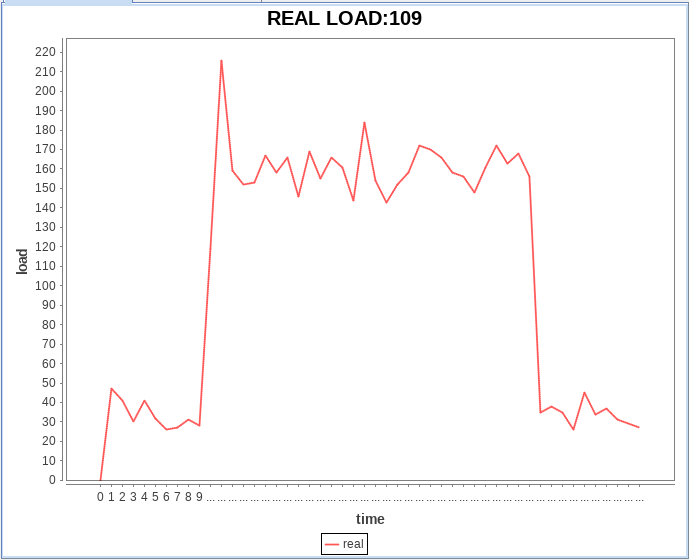
\includegraphics[scale=0.6]{grafico-carga-modulada2.png}
		\caption{Carga gerada com base nas configuração}
		\label{fig:grafico-carga-modulada2}
	\end{subfigure}
	\caption{Carga gerada com base na configuração: Degrau Negativo}
	\label{fig:carga-modulada2}
	\fautor
\end{figure}

A figura \ref{fig:carga-modulada2} apresenta os resultados dos parâmetros para o objetivo do Degrau Negativo. Os parâmetros de \textit{Base Load} e \textit{Duration} são os mesmos do experimento anterior, 30 EBs e 100 segundos de execução, conforme apresentado na figura \ref{fig:condiguracao-carga-bench4q2}. Já na \ref{fig:condiguracao-carga-modulada3} que demonstra os parâmetros utilizados para modular a carga, o \textit{Start Time} recebe o valor 0, assim a carga modulado iniciar com potência máxima utilizando os 30 EBs sendo 20 EBs setado no \textit{Quantity} para reservá-los para a modulação, o tempo de carga máxima é de 30 segundos como é possível ver no parâmetro \textit{Duration Step}, neste caso o \textit{Pause} é setado com 40 segundos, este valor é o que fará a interrupção brusca dos 20 EBs caindo o nível da geração de carga, gerando o degrau negativo. Passado esse período de pausa, a carga retorna ao seu nível máxima e atua por mais 30 segundos, o resultado final pode ser visto na figura \ref{fig:grafico-carga-modulada2}. 
%vale chamar a atenção para a dinâmica apresentada pela geração da carga sempre ao atingir o nivel maximo

\begin{figure}[!htb]
	\begin{subfigure}{\linewidth}
		\centering
		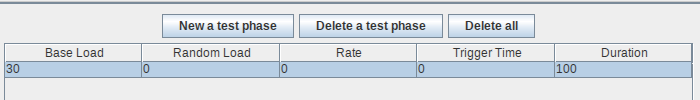
\includegraphics[scale=0.7]{condiguracao-carga-bench4q3.png}
		\caption{Configuração da carga no Bench4Q, para uma onda quadrada}
		\label{fig:condiguracao-carga-bench4q3}
	\end{subfigure}\\
	\begin{subfigure}{\linewidth}
		\centering
		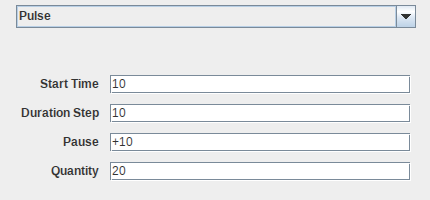
\includegraphics[scale=0.7]{condiguracao-carga-modulada3.png}
		\caption{Configuração para modular a carga como uma onda quadrada}
		\label{fig:condiguracao-carga-modulada3}
	\end{subfigure}\\[1ex]
	\begin{subfigure}{\linewidth}
		\centering
		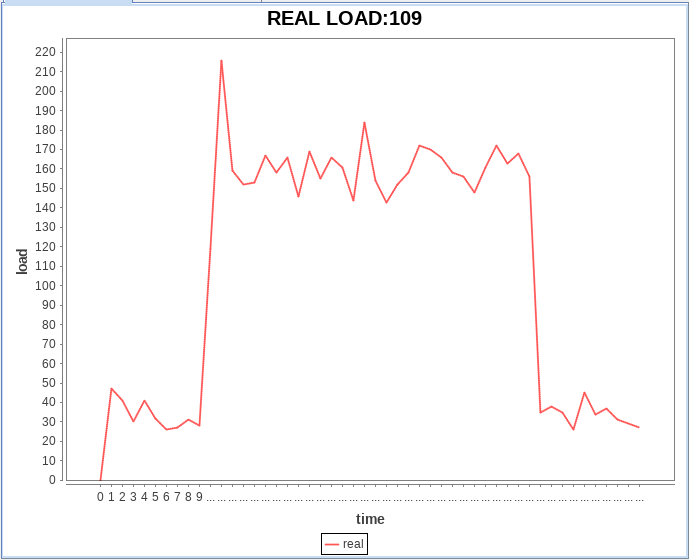
\includegraphics[scale=0.6]{grafico-carga-modulada3.png}
		\caption{Carga gerada com base nas configuração}
		\label{fig:grafico-carga-modulada3}
	\end{subfigure}
	\caption{Carga gerada com base na configuração: Onda Quadrada}
	\label{fig:carga-modulada3}
	\fautor
\end{figure}

Na figura \ref{fig:carga-modulada3} apresenta o resultado a modulação de uma onda quadrada, os parâmetros iniciais do Bench4Q referente a figura \ref{fig:condiguracao-carga-bench4q3} são os mesmos valores dos outros dois exemplos anteriores. Para gerar uma carga modula com comportamento oscilatório como a de uma onda quadrada, os parâmetros \ref{fig:condiguracao-carga-modulada3} são definidos com 10 segundos para \textit{Start Time}, 10 segundo de duração para \textit{Duration Step} e 10 para o \textit{Pause}, também configurado com 20 EBs. Para este exemplo vale salientar que para modular a carga como uma onda quadrada são dois parâmetros são importante e fundamentais \textit{Duration Step} e \textit{Pause}, estes devem ter os mesmos valores, pois eles é o quem manterão durante o período definido a carga em níveis baixo e máximo. 

%3º  - mostrar a analise e o impacto do carga de trabalho no sistema  
%Podemos agora usar os resultados da análise de desempenho para atender as metas estabelecidas no ponto 6.3.1. Por meio do modelo de QPN desenvolvido, que foram capazes de prever o desempenho do sistema em condições de funcionamento normais com 4 e 6 servidores WebLogic. Descobriu-se que usando o balanceador de carga original, seis nós de servidor de aplicação não foram suficientes para garantir tempos médios de resposta de transações de negócios abaixo de meio segundo. Atualizando o balanceador de carga com um CPU ligeiramente mais rápido levou à utilização de CPU do dropping balanceador de carga por um bom 20 por cento.
%Como resultado, os tempos de resposta de transações de concessionários melhorou em 15 a 27 por cento, encontrando o "meio segundo" exigência. No entanto, o aumento da intensidade da carga de trabalho além das condições de pico revelou que o balanceador de carga foi um recurso gargalo, impedindo-nos para escalar o sistema adicionando servidores WebLogic adicionais (veja a Figura 6.14). Assim, à luz do crescimento da carga de trabalho que o esperado, a empresa deve substituir a máquina balanceador de carga com um mais rápido ou considerar o uso de um método de balanceamento de carga mais eficiente. Depois de feito isso, a análise de desempenho deve ser repetida com o novo balanceador de carga para se certificar de que não há nenhum outro gargalos do sistema. Também deve ser assegurado que o balanceador de carga é configurado com threads suficientes para que não há contenção de discussão.
%Neste capítulo, a prática metodologia de modelagem de desempenho para DCS foi apresentada.
%A metodologia aproveita o poder de modelagem e expressividade do formalismo de modelagem QPN para melhorar a representatividade do modelo e permitir a previsão de desempenho precisas. Foi apresentado um estudo de caso detalhado no qual um modelo de um DCS realista foi construído e usado para analisar o seu desempenho e escalabilidade.
%O modelo de representatividade foi validado comparando suas previsões contra medições no sistema real. Foram considerados Um número de diferentes configurações de implantação e cenários de carga de trabalho. Além disso a CPU e I / O de contenção, demonstrou-se como alguns aspectos mais complexas do comportamento do sistema, tais como a contenção de rosca e processamento assíncrono, pode ser modelado. O modelo mostrou para refletir com precisão as características do sistema de desempenho e escalabilidade em estudo. O erro de modelagem para o tempo de resposta da transação não ultrapassou 21,2% e foi muito menor para a transferência de transações e utilização de recursos. A metodologia de modelagem de desempenho proposto fornece uma ferramenta poderosa para a engenharia de DCS desempenho.

%As análises apresentadas nessa Seção consideram a execução de rajadas de requisições dos usuários com e sem a presença de mecanismos de segurança, seguindo o planejamento definido na Seção anterior. Dessa forma, para uma melhor abordagem dos dados analisados, as avaliações foram divididas em duas Seções de acordo com o cenário.

\section{Contribuição}